\documentclass{beamer}
\usepackage{csc}
\title{Лекция 6. Наследование. Перегрузка операторов}

\date{
   \textbf{ИТМО JB}\\
   12 октября 2021 \\
   Санкт-Петербург
}

\begin{document}
\begin{frame} 
  \titlepage
\end{frame}

\begin{frame}[fragile]{Еще раз про множественное наследование}
    \emph{Множественное наследование (multiple inheritance)}~--- возможность
    наследовать сразу несколько классов.
\medskip
    \begin{lstlisting}
struct Unit {
    Unit(unitid id, int hp): id_(id), hp_(hp) {}
    virtual unitid id() const { return id_; }
    virtual int    hp() const { return hp_; }
private:
    unitid id_;
    int	   hp_;
};
    \end{lstlisting}
\end{frame}

\begin{frame}[fragile]{Еще раз про множественное наследование}
    \begin{lstlisting}
struct Elf:    Unit { ... };
struct Archer: Unit { ... };

struct ElfArcher: Elf, Archer {
    unitid id() const { return Elf::id(); }
    int    hp() const { return Elf::hp(); }
};
    \end{lstlisting}
\end{frame}

% % % % % % % % % % % % % % % % % % % % % % % % % % % % % % % % %
\begin{frame}[fragile]{Представление в памяти}
\begin{center}
\begin{tikzpicture}
   \begin{scope}[thick,
       block/.style={rectangle,draw,fill=cyan!20,minimum size=6mm,minimum width=1.3cm},
	   comp/.style={rectangle,draw,fill=orange!40, minimum size=6mm,minimum width=1.3cm}]
   \node [block] (re)	              				{ElfArcher};
   \node [comp]	 (st)	[above=of re,xshift=+1cm]	{Archer} edge [<-] (re);
   \node [comp]	 (em)	[above=of re,xshift=-1cm]	{Elf}  edge [<-] (re);
   \node [comp]	 (p1)	[above=of st]	            {Unit}   edge [<-] (st);
   \node [comp]	 (p2)	[above=of em]	            {Unit}   edge [<-] (em);
   \end{scope}
\end{tikzpicture}\hfill
\begin{tikzpicture}
\begin{scope}[start chain=1 going right,node distance=-0.15mm,yshift=-3cm]
    \tikzstyle{every path}=[thick]
    \tikzstyle{tmtape}=[draw,minimum height=6mm,fill=orange!40,minimum width=1.3cm]
    \node [on chain=1,tmtape] (p1) {Unit};
    \node [on chain=1,tmtape] (st) {Elf};
    \node [on chain=1,tmtape] (p2) {Unit};
    \node [on chain=1,tmtape] (em) {Archer};
    \node [on chain=1,tmtape,fill=cyan!20] (ea) {ElfArcher};
    \node [below=of p1, yshift=-1cm] (s1) {Elf}    edge [->] (p1.south west);
    \node [below=of s1] {ElfArcher};

    \node [below=of p2, yshift=-1cm] {Archer}    edge [->] (p2.south west);
\end{scope}
\end{tikzpicture}
\end{center}

\end{frame}


% % % % % % % % % % % % % % % % % % % % % % % % % % % % % % % % %
\begin{frame}[fragile]{Создание и удаление объекта}
\begin{center}
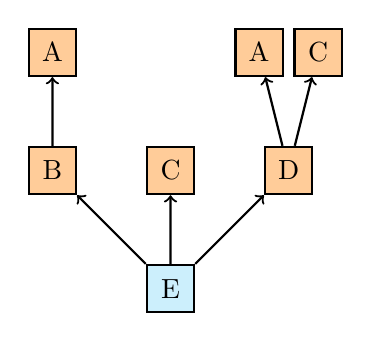
\begin{tikzpicture}[->,thick,
       block/.style={rectangle,draw,fill=cyan!20,minimum size=6mm},
	   comp/.style={rectangle,draw,fill=orange!40, minimum size=6mm},
	   level/.style={sibling distance = 1.5cm/#1, level distance = -1.5cm}]
   \node [block] (a1) {E} 
       child {node [comp] {B}
               child {node [comp] {A}}} 
       child {node [comp] {C}} 
       child {node [comp] {D} 
               child {node [comp] {A}}
               child {node [comp] {C}}};
\end{tikzpicture}
\end{center}


Порядок вызова конструкторов: \texttt{A, B, C, A, C, D, E}.

Деструкторы вызываются в обратном порядке.

Проблемы:
\begin{enumerate}
    \item Дублирование \texttt{A} и \texttt{C}.
    \item Недоступность первого \texttt{C}.
\end{enumerate}

\end{frame}

% % % % % % % % % % % % % % % % % % % % % % % % % % % % % % % % %
\begin{frame}[fragile]{Виртуальное наследование}

\begin{center}
\begin{tikzpicture}[thick,
		block/.style={rectangle,draw,fill=cyan!20,minimum size=6mm,minimum width=1.5cm},
		comp/.style={rectangle,draw,fill=orange!40, minimum size=6mm,minimum width=1.5cm}]
   \node [block] (so)					{Song};
   \node [comp]	 (ly)	[above=of re,xshift=-1cm]	{Lyrics}        edge [<-] (so);
   \node [comp]	 (mu)	[above=of re,xshift=+1cm]	{Music}         edge [<-] (so);
   \node [comp]	 (aw1)	[above=of ly]	            {ArtWork}       edge [<-] (ly);
   \node [comp]	 (aw2)	[above=of mu]	            {ArtWork}       edge [<-] (mu);
\end{tikzpicture}\hspace{2cm}
\begin{tikzpicture}[thick,
		block/.style={rectangle,draw,fill=cyan!20,minimum size=6mm,minimum width=1.5cm},
		comp/.style={rectangle,draw,fill=orange!40, minimum size=6mm,minimum width=1.5cm}]
   \node [block] (so)					            {ElfArcher};
   \node [comp]	 (ly)	[above=of re,xshift=-1cm]	{Elf}        edge [<-] (so);
   \node [comp]	 (mu)	[above=of re,xshift=+1cm]	{Archer}       edge [<-] (so);
   \node<1> [comp]	 (aw1)	[above=of ly,xshift=+1cm]   {Unit}  
        edge [<-] node [color=black,xshift= 6mm] {} (mu)
        edge [<-] node [color=black,xshift=-6mm] {} (ly);
   \node<2> [comp]	 (aw1)	[above=of ly,xshift=+1cm]   {Unit}  
           edge [<-,color=red] node [color=black,xshift= 6mm] {\color{MOOCBlue}{virtual}} (mu)
           edge [<-,color=red] node [color=black,xshift=-6mm] {\color{MOOCBlue}{virtual}} (ly);
\end{tikzpicture}
\end{center}
\pause

    \begin{lstlisting}
struct Unit {};
struct Elf:  virtual Unit {};
struct Archer: virtual Unit {};
struct ElfArcher: Elf, Archer {};
    \end{lstlisting}
\end{frame}

% % % % % % % % % % % % % % % % % % % % % % % % % % % % % % % % %
\begin{frame}[fragile]{Как устроено расположение в памяти?}{}
\vspace{4pt}
\parbox{4cm}{
\begin{tikzpicture}[thick,
		block/.style={rectangle,draw,fill=cyan!20,minimum size=6mm,minimum width=1.5cm},
		comp/.style={rectangle,draw,fill=orange!40, minimum size=6mm,minimum width=1.5cm}]
   \node [block] (so)					            {ElfArcher};
   \node [comp]	 (ly)	[above=of re,xshift=-1cm]	{Elf}        edge [<-] (so);
   \node [comp]	 (mu)	[above=of re,xshift=+1cm]	{Archer}       edge [<-] (so);
   \node [comp]	 (aw1)	[above=of ly,xshift=+1cm]   {Unit}  
        edge [<-,color=red] node [color=black,xshift= 6mm] {\color{MOOCBlue}{virtual}} (mu)
        edge [<-,color=red] node [color=black,xshift=-6mm] {\color{MOOCBlue}{virtual}} (ly);
\end{tikzpicture}}\parbox{6cm}{
\begin{tikzpicture}
    \tikzstyle{every path}=[thick]
    \tikzstyle{tmtape}=[draw,minimum height=6mm, minimum width=1.5cm]
\begin{scope}[start chain=1 going right,node distance=-0.15mm]
    \node [on chain=1,tmtape,draw=none, minimum width=25mm] {Elf};
    \node [on chain=1,tmtape] {Unit};
    \node [on chain=1,tmtape] {Elf};
\end{scope}
\begin{scope}[start chain=1 going right,node distance=-0.15mm,yshift=-1cm]
    \node [on chain=1,tmtape,draw=none, minimum width=25mm] {Archer};
    \node [on chain=1,tmtape] {Unit};
    \node [on chain=1,tmtape] {Archer};
\end{scope}
\begin{scope}[start chain=1 going right,node distance=-0.15mm,yshift=-2cm]
    \node [on chain=1,tmtape,draw=none, minimum width=25mm] {ElfArcher?};
    \node [on chain=1,tmtape] {Unit};
    \node [on chain=1,tmtape] {Elf};
    \node [on chain=1,tmtape] {Archer};
\end{scope}
\begin{scope}[start chain=1 going right,node distance=-0.15mm,yshift=-3cm]
    \node [on chain=1,tmtape,draw=none, minimum width=25mm] {ElfArcher?};
    \node [on chain=1,tmtape] {Elf};
    \node [on chain=1,tmtape] {Unit};
    \node [on chain=1,tmtape] {Archer};
\end{scope}
\end{tikzpicture}}
\vskip5mm\pause

\parbox{4cm}{
На самом деле.}\parbox{6cm}{
\begin{tikzpicture}
    \tikzstyle{every path}=[thick]
    \tikzstyle{tmtape}=[draw,minimum height=6mm, minimum width=1.5cm]
\begin{scope}[start chain=1 going right,node distance=-0.15mm]
    \node [on chain=1,tmtape,draw=none, minimum width=25mm] {Elf};
    \node [on chain=1,tmtape] {Elf};
    \node [on chain=1,tmtape] {Unit};
\end{scope}
\begin{scope}[start chain=1 going right,node distance=-0.15mm,yshift=-1cm]
    \node [on chain=1,tmtape,draw=none, minimum width=25mm] {Archer};
    \node [on chain=1,tmtape] {Archer};
    \node [on chain=1,tmtape] {Unit};
\end{scope}
\begin{scope}[start chain=1 going right,node distance=-0.15mm,yshift=-2cm]
    \tikzstyle{every path}=[thick]
    \tikzstyle{tmtape}=[draw,minimum height=6mm, minimum width=1.5cm]
    \node [on chain=1,tmtape,draw=none, minimum width=25mm] {ElfArcher};
    \node [on chain=1,tmtape] {Elf};
    \node [on chain=1,tmtape] {Archer};
    \node [on chain=1,tmtape] {Unit};
\end{scope}
\end{tikzpicture}}
\end{frame}

% % % % % % % % % % % % % % % % % % % % % % % % % % % % % % % % %
\begin{frame}[fragile]{Доступ через таблицу виртуальных методов}
    \begin{lstlisting}
struct Unit { 
    unitid id;
};
struct Elf  : virtual Unit { };
struct Archer : virtual Unit { };
struct ElfArcher : Elf, Archer { };
    \end{lstlisting}
Рассмотрим такой код:
    \begin{lstlisting}
    Elf * e = (rand() % 2)? new Elf() : new ElfArcher();
    unitid id = e->id; // (*)
    \end{lstlisting}
Строка \texttt{(*)} будет преобразована в строку
    \begin{lstlisting}
    unitid id = e->__getUnitPtr__()->id;
    \end{lstlisting}
где \texttt{\_\_getUnitPtr\_\_()}~— это служебный виртуальный метод.
\end{frame}


% % % % % % % % % % % % % % % % % % % % % % % % % % % % % % % % %
\begin{frame}[fragile]{Кто вызывает конструктор базового класса?}
\begin{minipage}{.6\textwidth}
    \begin{lstlisting}
struct Unit { 
    Unit() = default;
    Unit(unitid id, int health); 
};
struct Elf: virtual Unit {
    explicit Elf(unitid id) 
        : Unit(id, 100) {}
};
struct Archer: virtual Unit {
    explicit Archer(unitid id) 
        : Unit(id, 120) {}
};
struct ElfArcher: Elf, Archer {
    explicit ElfArcher(unitid id) 
        : Elf(id)
        , Archer(id) {}
};
    \end{lstlisting}
\end{minipage}\hspace{10mm}
\begin{minipage}{.25\textwidth}
\begin{tikzpicture}[thick,
		block/.style={rectangle,draw,fill=cyan!20,minimum size=6mm,minimum width=1.5cm},
		comp/.style={rectangle,draw,fill=orange!40, minimum size=6mm,minimum width=1.5cm}]
   \node [block] (so)					            {ElfArcher};
   \node [comp]	 (ly)	[above=of re,xshift=-1cm]	{Elf}        edge [<-] (so);
   \node [comp]	 (mu)	[above=of re,xshift=+1cm]	{Archer}       edge [<-] (so);
   \node [comp]	 (aw1)	[above=of ly,xshift=+1cm]   {Unit}  
           edge [<-,color=red] node [color=black,xshift= 6mm] {\color{MOOCBlue}{virtual}} (mu)
           edge [<-,color=red] node [color=black,xshift=-6mm] {\color{MOOCBlue}{virtual}} (ly);
\end{tikzpicture}
\end{minipage}

\end{frame}

\begin{frame}[fragile]{Кто вызывает конструктор базового класса?}
        \begin{lstlisting}
struct Unit { 
    // Unit() = default;
    Unit(unitid id, int health); 
};
struct Elf: virtual Unit {
    explicit Elf(unitid id) 
        : Unit(id, 100) {}
};
struct Archer: virtual Unit {
    explicit Archer(unitid id) 
        : Unit(id, 120) {}
};
struct ElfArcher: Elf, Archer {
    explicit ElfArcher(unitid id) 
        : Elf(id)
        , Archer(id) {}
};
        \end{lstlisting}
    Ошибка компиляции: не вызван соответствующий конструктор.
\end{frame}

\begin{frame}[fragile]{Кто вызывает конструктор базового класса?}
    \begin{lstlisting}
struct Unit { 
    Unit(unitid id, int health); 
};
struct Elf: virtual Unit {
    explicit Elf(unitid id) 
        : Unit(id, 100) {}
};
struct Archer: virtual Unit {
    explicit Archer(unitid id) 
        : Unit(id, 120) {}
};
struct ElfArcher: Elf, Archer {
    explicit ElfArcher(unitid id) 
        : Unit(id, 150)
        , Elf(id)
        , Archer(id) {}
};
    \end{lstlisting}
\end{frame}

% % % % % % % % % % % % % % % % % % % % % % % % % % % % % % % % %
\begin{frame}[fragile]{Заключение}
    \begin{itemize}
        \item Не используйте множественное наследование для наследования
            реализации.
        
        \item Используйте концепцию интерфейсов (классы без реализаций и членов данных).

        \item Помните о неприятностях, связанных с множественным наследованием.

        \item Хорошо подумайте перед тем, как использовать виртуальное
            наследование.

        \item Помните о неприятностях, связанных с виртуальным наследованием.
    \end{itemize}
\end{frame}

\begin{frame}[fragile]{Основные операторы}
    \begin{block}{Арифметические}
        \begin{itemize}
            \item Унарные: префиксные {\color{blue}\verb!+ - ++ --!},
                постфиксные {\color{blue}\verb!++ --!}
            \item Бинарные: {\color{blue}\verb!+ - * / % += -= *= /= %=!}
        \end{itemize}
    \end{block}
    \begin{block}{Битовые}
        \begin{itemize}
            \item Унарные: {\color{blue}\verb!~!}.
            \item Бинарные: {\color{blue}\verb!& | ^ &= |= ^= >> << >>= <<=!}.
        \end{itemize}
    \end{block}
    \begin{block}{Логические}
        \begin{itemize}
            \item Унарные: {\color{blue}\verb#!#}. 
            \item Бинарные: {\color{blue}\verb!&& ||!}.
            \item Сравнения: {\color{blue}\verb#== != > < >= <=#}
            \item C++20: {\color{blue}\verb#<=>#}
        \end{itemize}
    \end{block}
\end{frame}

\begin{frame}[fragile]{Другие операторы}
        \begin{enumerate}
            \item Оператор присваивания: {\color{blue}\verb!=!}
            \item Специальные: 
                \begin{itemize}
                    \item префиксные {\color{blue}\verb!* &!}, 
                    \item постфиксные  {\color{blue}\verb!-> ->*!}, 
                    \item особые {\color{blue}\verb!,! \verb!. .* ::!}
                \end{itemize}
            \item Скобки: {\color{blue}\verb![] ()!}
            \item Оператор приведения {\color{blue} \verb!(type)!}
            \item Тернарный оператор: {\color{blue}\verb! x ? y : z !}
            \item Работа с памятью: {\color{blue}\verb!new new[] delete delete[]!}
        \end{enumerate}

    Нельзя перегружать операторы {\color{blue}\verb!.! \verb!::!} и тернарный
    оператор.
\end{frame}

\begin{frame}[fragile]{Перегрузка операторов}
    \begin{lstlisting}
Vector operator-(Vector const& v) {
    return Vector(-v.x, -v.y)
}

Vector operator+(Vector const& v, 
                 Vector const& w) {
    return Vector(v.x + w.x, v.y + w.y);
}

Vector operator*(Vector const& v, double d) {
    return Vector(v.x * d, v.y * d);
}

Vector operator*(double d, Vector const& v) {
    return v * d;
}
    \end{lstlisting}
\end{frame}

\begin{frame}[fragile]{Перегрузка операторов внутри классов}
    {}\small\textbf{NB:} Обязательно для {\color{blue}\verb!(type) [] () -> ->* =!}

    \begin{lstlisting}[basicstyle=\fontsize{9pt}{1em}\ttfamily]
struct Vector {
    Vector operator-() const { return Vector(-x, -y); }
    Vector operator-(Vector const& p) const {
        return Vector(x - p.x, y - p.y);
    }
    Vector & operator*=(double d) {
        x *= d;
        y *= d;
        return *this;
    }
    double operator[](size_t i) const { 
        return (i == 0) ? x : y;
    }
    bool    operator()(double d)   const   { ... }
    void    operator()(double a, double b) { ... }
    double x, y;
};
    \end{lstlisting}
\end{frame}

\begin{frame}[fragile]{Перегрузка инкремента и декремента}
    \begin{lstlisting}
struct BigNum {
    BigNum & operator++() { //prefix
        //increment
        ...
        return *this;
    }

    BigNum operator++(int) { //postfix
        BigNum tmp(*this);
        ++(*this);
        return tmp;
    }
    ...
};
    \end{lstlisting}
\end{frame}

\begin{frame}[fragile]{Переопределение операторов ввода-вывода}
    \begin{lstlisting}
#include <iostream>
        
struct Vector { ... };

std::istream& operator>>(std::istream & is, 
                         Vector & p) {
    is >> p.x >> p.y;
    return is;
}

std::ostream& operator<<(std::ostream &os, 
                         Vector const& p) {
    os << p.x << ' ' <<  p.y;
    return os;
}
    \end{lstlisting}
\end{frame}

\begin{frame}[fragile]{Умный указатель}
Реализует принцип: {\em ``Получение ресурса есть инициализация''
Resource Acquisition Is Initialization (RAII)}
\begin{lstlisting}
struct SmartPtr {
   Data & operator*()  const {return *data_;}
   Data * operator->() const {return  data_;}
   Data * get()        const {return  data_;}
   ... 
private:
   Data * data_;
};

bool operator==(SmartPtr const& p1,
                SmartPtr const& p2) {
    return p1.get() == p2.get();
}
    \end{lstlisting}
\end{frame}

\begin{frame}[fragile]{Умный указатель}
    \begin{lstlisting}
struct Data { int id; };

struct SmartPtr {
    Data & operator*()  const {return *data_;}
    Data * operator->() const {return  data_;}
    Data * get()        const {return  data_;}
    ... 
private:
    Data * data_;
};

SmartPtr p;
p->id; // p.operator->()->id;
p->foo() // error
        \end{lstlisting}
\end{frame}

\begin{frame}[fragile]{Указатели на функции}
    Кроме указателей на значения в \texttt{C++} присутствуют три особенных 
    типа указателей:
    \begin{enumerate}
        \item указатели на функции (унаследованно из \texttt{C}),
        \item указатели на методы,
        \item указатели на поля классов.
    \end{enumerate}
    
    Указатели на функции (и методы) используются для
    \begin{enumerate}
        \item параметризация алгоритмов,
        \item обратных вызовов (callback),
        \item подписки на события (шаблон Listener),
        \item создание очередей событий/заданий.
    \end{enumerate}
\end{frame}

\begin{frame}[fragile]{Указатели на функции: параметризация алгоритмов}
    \begin{lstlisting}
bool less(double a, double b) { return a < b; }

void sort(double * p, double * q,
          bool (*cmp)(double, double)) {
    for (double * m = p; m != q; ++m)
        for (double * r = m; r + 1 != q; ++r)
            if ( cmp(*(r + 1), *r) )
                swap(*r, *(r + 1));
}
int main() {
    double m[100];
    sort(m, m + 100, &less);
}
    \end{lstlisting}
\end{frame}
 
\begin{frame}[fragile]{Сразу о полезности \texttt{using}}
Что здесь объявлено?
    \begin{lstlisting}
char * (*func(int, int))(int, int, int *, float);
    \end{lstlisting}

Функция двух целочисленных параметров, возвращающая указатель на функцию,
которая возвращает указатель на \texttt{char} и имеет собственный список
формальных параметров вида: \texttt{(int, int, int *, float)}

\medskip

Как стоило это написать:
    \begin{lstlisting}
using SomeFunction 
    = std::function<char*(int, int, int *, float)>;
SomeFunction func(int, int);
    \end{lstlisting}
\end{frame}

\begin{frame}[fragile]{Указатели на методы}
\small
В отличие от указателей на функции требуют экземпляр класса.
    \begin{lstlisting}
struct Person {
    string name() const;
    string surname() const;
};
using MPTR = string (Person::*)() const;

void print(Person const& p) {
    static MPTR im[2] = {
        &Person::name, 
        &Person::surname};

    for (size_t i = 0; i != 3; ++i)
        cout << (p.*im[i])(); // operator .*
}
    \end{lstlisting}
\end{frame}


\begin{frame}[fragile]{Указатели на члены данных}
\small
    Похожи на указатели на методы.
    \begin{lstlisting}
struct Person {
    string name;
    string surname;
};

using DPTR = string Person::*;

void print(Person const& p) {
    static DPTR im[2] = {
        &Person::name,
        &Person::surname};

    for (size_t i = 0; i != 3; ++i)
        cout << (p.*im[i]); // operator .*
}
    \end{lstlisting}
\end{frame}

\begin{frame}[fragile]{Резюме по синтаксису}
Указатели на методы и поля класса. 
    \begin{lstlisting}
struct Student { 
    string name () const { return name_; } 
    string name_;
};
int main() {
    string (Student::*mptr)() const = &Student::name;
    string  Student::*dptr          = &Student::name_;
    Student s;
    Student * p = &s;
    (s.*mptr)() == (p->*mptr)();
    (s.*dptr)   == (p->*dptr);
}
    \end{lstlisting}
\end{frame}

\begin{frame}[fragile]{Резюме по синтаксису}
    \begin{lstlisting}
struct Foo {
    int i;
    void f();
};

int main () {
    Foo foo;
    Foo* fooPtr = &foo;
    int Foo::* iPtr = &Foo::i;
    void (Foo::*memFuncPtr)() = &Foo::f;

    foo.*iPtr = 0;
    fooPtr->*iPtr = 0;
    (foo.*memFuncPtr)();
    (fooPtr->*memFuncPtr)();
}
    \end{lstlisting}
\end{frame}

\begin{frame}[fragile]{Резюме по синтаксису}
    Начиная с С++17 для вызова функций по указателю удобно использовать \code{std::invoke}.
    \begin{lstlisting}
int main() {
    Foo foo;
    Foo* fooPtr = &foo;
    auto iPtr = &Foo::i;
    auto memFuncPtr = &Foo::f;

    std::invoke(iPtr, foo) = 0;
    std::invoke(iPtr, fooPtr) = 0;

    std::invoke(memFuncPtr, foo);
    std::invoke(memFuncPtr, fooPtr);
}
    \end{lstlisting}
\end{frame}

\begin{frame}[fragile]{Оператор ->*}
    \begin{lstlisting}
template<typename ItemType>
struct List {
    List(ItemType *head,
         ItemType * ItemType::*nextMemPointer)
    : m_head(head)
    , m_nextMemPointer(nextMemPointer) { }

    void addHead(ItemType *item) {
    (item ->* m_nextMemPointer) = m_head;
    m_head = item;
    }

private:
    ItemType *m_head;
    ItemType * ItemType::*m_nextMemPointer;
};
    \end{lstlisting}
\end{frame}

\begin{frame}[fragile]{Оператор приведения}
    \begin{lstlisting}
struct String {
    operator bool() const {
        return size_ != 0;
    }

    operator char const *() const {
        if (*this)
            return data_;
        return "";
    }

private:
    char * data_;
    size_t size_;
};
    \end{lstlisting}
\end{frame}

\begin{frame}[fragile]{Операторы с особым порядком вычисления}
    \begin{lstlisting}
int main() {
    int a = 0;
    int b = 5;
    (a != 0) && (b = b / a);
    (a == 0) || (b = b / a);

    foo() && bar();
    foo() || bar();
    foo(), bar();
}
    \end{lstlisting}
\end{frame}

\begin{frame}[fragile]{Операторы с особым порядком вычисления}
    \begin{lstlisting}
struct P
{
    int data = 0;
};

// no lazy semantics
Tribool operator&&(Tribool const& b1, 
                   Tribool const& b2);

int main() {
    P * p = new P();
    // lazy semantics
    if (p && p->data)
    {
         ...
    }
}
    \end{lstlisting}
\end{frame}

\begin{frame}[fragile]{Переопределение арифметических операторов}
    \begin{lstlisting}
struct String {
    String( char const * cstr ) { ... }
    String & operator+=(String const& s) {
        ...
        return *this;    
    }
    //\verb!String operator+(String const& s2) const {...}!
};
String operator+(String s1, String const& s2) { 
    return s1 += s2; 
}
    \end{lstlisting}
    \begin{lstlisting}
    String s1("world");
    String s2 = "Hello " + s1;
    \end{lstlisting}
\end{frame}

\begin{frame}[fragile]{``Правильное'' переопределение операторов сравнения}
    \begin{lstlisting}[basicstyle=\fontsize{9pt}{1em}\ttfamily]
bool operator==(String const& a, String const& b) 
{ return ...  }
bool operator!=(String const& a, String const& b) 
{ return !(a == b); }

bool operator<(String const& a, String const& b) 
{ return ...  }
bool operator>(String const& a, String const& b) 
{ return b < a; }
bool operator<=(String const& a, String const& b) 
{ return !(b < a); }
bool operator>=(String const& a, String const& b) 
{ return !(a < b); }
    \end{lstlisting}
\end{frame}

\begin{frame}[fragile]{C++20 переопределение операторов сравнения}
    \begin{lstlisting}[basicstyle=\fontsize{9pt}{1em}\ttfamily]
struct Record
{
    std::string name;
    unsigned int floor;
    double weight;
    auto operator<=>(const Record&) const = default;
};

// now can be compared with ==, !=, <, <=, >, and >=
    \end{lstlisting}
\end{frame}

\begin{frame}[fragile]{C++20 переопределение операторов сравнения}
    \begin{lstlisting}[basicstyle=\fontsize{9pt}{1em}\ttfamily]
struct Base {
    std::string zip;
    auto operator<=>(const Base&) const = default;
};
struct TotallyOrdered : Base {
    std::string tax_id;
    std::string first_name;
    std::string last_name;
public:
    // custom operator<=> because we want to compare last names first
    std::strong_ordering operator<=>(
        const TotallyOrdered& that) const;
};
    \end{lstlisting}
\end{frame}

\begin{frame}[fragile]{C++20 переопределение операторов сравнения}
    \begin{lstlisting}[basicstyle=\fontsize{9pt}{1em}\ttfamily]
std::strong_ordering TotallyOrdered::operator<=>(
    const TotallyOrdered& that) const {
    if (auto cmp = (Base&)(*this) <=> (Base&)that; cmp != 0)
        return cmp;
    if (auto cmp = last_name <=> that.last_name; cmp != 0)
        return cmp;
    if (auto cmp = first_name <=> that.first_name; cmp != 0)
        return cmp;
    return tax_id <=> that.tax_id;
}
    \end{lstlisting}
\end{frame}

\begin{frame}[fragile]{О чём стоит помнить}
    \begin{itemize}
        \item Стандартная семантика операторов.
\begin{lstlisting}
void operator+(A const & a, A const& b) {}
\end{lstlisting}
        \item Приоритет операторов.
\begin{lstlisting}
    Vector a, b, c;
    c = a + a ^ b * a; //?????
\end{lstlisting}
    \item Хотя бы один из параметров должен быть пользовательским.
\begin{lstlisting}
    void operator*(double d, int i) {}
\end{lstlisting}
    \end{itemize}
\end{frame}

\end{document}

 
